%% Преамбула TeX-файла

% 1. Стиль и язык
 \documentclass[utf8x, 14pt]{G7-32}

% \newfontfamily{\FA}{[FontAwesome.otf]}
% \usepackage{graphicx}
% \documentclass[utf8x, times, 14pt]{G7-32}

%% Стиль (по умолчанию будет 14pt)

% Остальные стандартные настройки убраны в preamble.inc.tex.
\sloppy
% Настройки стиля ГОСТ 7-32
% Для начала определяем, хотим мы или нет, чтобы рисунки и таблицы нумеровались в пределах раздела, или нам нужна сквозная нумерация.
\EqInChapter % формулы будут нумероваться в пределах раздела
\TableInChapter % таблицы будут нумероваться в пределах раздела
\PicInChapter % рисунки будут нумероваться в пределах раздела

% Добавляем гипертекстовое оглавление в PDF
\usepackage[
bookmarks=true, colorlinks=true, unicode=true,
urlcolor=black,linkcolor=black, anchorcolor=black,
citecolor=black, menucolor=black, filecolor=black,
]{hyperref}

\AfterHyperrefFix

% добавил для оформления алгоритмов
% вариант 1
%\usepackage{algorithm2e}
% вариант 2
\usepackage{algorithm}
\usepackage{algpseudocode}
% для таблиц
\usepackage{ctable}% http://ctan.org/pkg/ctable
\usepackage{caption}% http://ctan.org/pkg/caption



\usepackage{microtype}% полезный пакет для микротипографии, увы под xelatex мало чего умеет, но под pdflatex хорошо улучшает читаемость

% Тире могут быть невидимы в Adobe Reader
\ifInvisibleDashes
\MakeDashesBold
\fi

\usepackage{graphicx}   % Пакет для включения рисунков

% С такими оно полями оно работает по-умолчанию:
% \RequirePackage[left=20mm,right=10mm,top=20mm,bottom=20mm,headsep=0pt,includefoot]{geometry}
% Если вас тошнит от поля в 10мм --- увеличивайте до 20-ти, ну и про переплёт не забывайте:
\geometry{right=20mm}
\geometry{left=30mm}
\geometry{bottom=20mm}
\geometry{ignorefoot}% считать от нижней границы текста


% Пакет Tikz
\usepackage{tikz}
\usetikzlibrary{arrows,positioning,shadows}

% Произвольная нумерация списков.
\usepackage{enumerate}

% ячейки в несколько строчек
\usepackage{multirow}

% itemize внутри tabular
\usepackage{paralist,array}

%\setlength{\parskip}{1ex plus0.5ex minus0.5ex} % разрыв между абзацами
\setlength{\parskip}{1ex} % разрыв между абзацами
\usepackage{blindtext}

% Центрирование подписей к плавающим окружениям
%\usepackage[justification=centering]{caption}

\usepackage{newfloat}
\DeclareFloatingEnvironment[
placement={!ht},
name=Equation
]{eqndescNoIndent}
\edef\fixEqndesc{\noexpand\setlength{\noexpand\parindent}{\the\parindent}\noexpand\setlength{\noexpand\parskip}{\the\parskip}}
\newenvironment{eqndesc}[1][!ht]{%
    \begin{eqndescNoIndent}[#1]%
\fixEqndesc%
}
{\end{eqndescNoIndent}}




% Настройки листингов.
\ifPDFTeX
% 8 Листинги

\usepackage{listings}

% Значения по умолчанию
\lstset{
  basicstyle= \footnotesize,
  breakatwhitespace=true,% разрыв строк только на whitespacce
  breaklines=true,       % переносить длинные строки
%   captionpos=b,          % подписи снизу -- вроде не надо
  inputencoding=koi8-r,
  numbers=left,          % нумерация слева
  numberstyle=\footnotesize,
  showspaces=false,      % показывать пробелы подчеркиваниями -- идиотизм 70-х годов
  showstringspaces=false,
  showtabs=false,        % и табы тоже
  stepnumber=1,
  tabsize=4,              % кому нужны табы по 8 символов?
  frame=single
}

% Стиль для псевдокода: строчки обычно короткие, поэтому размер шрифта побольше
\lstdefinestyle{pseudocode}{
  basicstyle=\small,
  keywordstyle=\color{black}\bfseries\underbar,
  language=Pseudocode,
  numberstyle=\footnotesize,
  commentstyle=\footnotesize\it
}

% Стиль для обычного кода: маленький шрифт
\lstdefinestyle{realcode}{
  basicstyle=\scriptsize,
  numberstyle=\footnotesize
}

% Стиль для коротких кусков обычного кода: средний шрифт
\lstdefinestyle{simplecode}{
  basicstyle=\footnotesize,
  numberstyle=\footnotesize
}

% Стиль для BNF
\lstdefinestyle{grammar}{
  basicstyle=\footnotesize,
  numberstyle=\footnotesize,
  stringstyle=\bfseries\ttfamily,
  language=BNF
}

% Определим свой язык для написания псевдокодов на основе Python
\lstdefinelanguage[]{Pseudocode}[]{Python}{
  morekeywords={each,empty,wait,do},% ключевые слова добавлять сюда
  morecomment=[s]{\{}{\}},% комменты {а-ля Pascal} смотрятся нагляднее
  literate=% а сюда добавлять операторы, которые хотите отображать как мат. символы
    {->}{\ensuremath{$\rightarrow$}~}2%
    {<-}{\ensuremath{$\leftarrow$}~}2%
    {:=}{\ensuremath{$\leftarrow$}~}2%
    {<--}{\ensuremath{$\Longleftarrow$}~}2%
}[keywords,comments]

% Свой язык для задания грамматик в BNF
\lstdefinelanguage[]{BNF}[]{}{
  morekeywords={},
  morecomment=[s]{@}{@},
  morestring=[b]",%
  literate=%
    {->}{\ensuremath{$\rightarrow$}~}2%
    {*}{\ensuremath{$^*$}~}2%
    {+}{\ensuremath{$^+$}~}2%
    {|}{\ensuremath{$|$}~}2%
}[keywords,comments,strings]

% Подписи к листингам на русском языке.
\renewcommand\lstlistingname{Листинг}
\renewcommand\lstlistlistingname{Листинги}

\else
\usepackage{local-minted}
\fi

% Полезные макросы листингов.
% Любимые команды
\newcommand{\Code}[1]{\textbf{#1}}


% Стиль титульного листа и заголовки
% \include{00-title}


\begin{document}

\frontmatter % выключает нумерацию ВСЕГО; здесь начинаются ненумерованные главы: реферат, введение, глоссарий, сокращения и прочее.

% \maketitle %создает титульную страницу


% \begin{executors}
% \personalSignature{Первый исполнитель}{ФИО}

% \personalSignature{Второй исполнитель}{ФИО}
% \end{executors}


%\listoffigures                         % Список рисунков

%\listoftables                          % Список таблиц

%\NormRefs % Нормативные ссылки 
% Команды \breakingbeforechapters и \nonbreakingbeforechapters
% управляют разрывом страницы перед главами.
% По-умолчанию страница разрывается.

% \nobreakingbeforechapters
% \breakingbeforechapters

% \include{00-abstract}

\tableofcontents

\printnomenclature % Автоматический список сокращений

% \include{12-intro}

\mainmatter % это включает нумерацию глав и секций в документе ниже

\setcounter{page}{2}

\chapter{Обзор}
\label{cha:owerview}
Обзоры по численному анализу ГРП можно найти в \cite{GuptaDiss2016, WeberDiss2016, Lecampion2018}. В \cite{Kolawole2020} рассматривается пересечение трещины гидроразрыва с естественными трещинами. Обзор XFEM есть в \cite{PereiraDiss2010,Belytschko2009,Fries2010,Karihaloo2011,Fries2014,flemisch2016,Ahmadkanth2019}.

Литература по моделированию ГРП с применением XFEM в трёхмерной постановке: 
\cite{Gupta2014,Zielonka2014,Gupta2015,GuptaDiss2016,Liu2016,Weber2016,Haddad2016,Gupta2017,Liu2017,Luo2018,Paul2018,Duarte2019,Duarte2020_validation,Duarte2020,Roth2020_1,Roth2020_2,Shi2021}.
\section{Гидравлический разрыв пласта}
Гидравлический разрыв пласта (ГРП) \cite{Magadova2012} -- это физико-гидродинамический процесс, при котором горная порода разрывается по плоскостям минимальной прочности за счет воздействия на пласт давлением, создаваемым закачкой в скважину специальной жидкости разрыва. В образованные трещины с помощью жидкостей разрыва транспортируется расклинивающий материал -- проппант, который, после снятия избыточного давления, закрепляет трещины в раскрытом состоянии. После разрыва давление флюида увеличивает размеры трещины, обеспечивая ее связь с системой естественных природных трещин, не вскрытых скважиной, а также с зонами повышенной проницаемости, расширяя таким образом площадь дренажа скважины и способствуя значительному увеличению ее дебита или приемистости на объектах нагнетания с повышением конечной нефтеотдачи продуктивных пластов.

Цели и области применения ГРП:
\renewcommand{\labelitemi}{$\bullet$}
\begin{itemize}
\item
интенсификация добычи из скважин, в первую очередь с интенсивно кольматированной призабойной зоной, увеличение эффективного радиуса за счет создания высокопроводящих трещин ограниченной длины в средне- и высокопроницаемых пластах, а также в низкопроницаемых достаточно однородных коллекторах;
\item
обеспечение гидродинамической связи скважины с системой естественных трещин пласта и расширение зоны дренирования;
\item
ввод в разработку низкопроницаемых залежей с потенциальным дебитом скважин в 2-3 раза ниже уровня рентабельной добычи и перевод забалансовых запасов в промышленные;
\item
разработка сложных расчлененных и неоднородных пластов, характеризующихся высокой степенью прерывистости, на основе комплексной оптимизации системы разработки с целью обеспечения гидродинамического взаимодействия пласта и системы скважин с трещинами гидраразрыва для увеличения темпа отбора извлекаемых запасов, повышения нефтеотдачи за счет вовлечения в активную разработку слабодренируемых зон и прослоев и увеличения охвата пласта воздействием.
\end{itemize}

Кислотный ГРП предполагает последовательный разрыв пласта полисахарядным гелем и закачку кислотного состава. В качестве жидкости для гидраразрыва могут использоваться прямые и обратные кислотосодержащие эмульсии или полимерные кислотные гели на водной основе.

При обычном ГРП скорость нагружения пород не превышает $1$ МПа/с, а в результате локального взрыва (импульсный ГРП) достигает $10^7$ МПа/с с чередующейся серией затухающих гидраударов скважинной жидкости. В настоящее время существует ряд методов создания щадящих пролонгированных взрывов в скважине с импульсами давления $10^1-10^7$ МПа/с. Как правило, импульсный разрыв формирует сеть горизонтальных коротких трещин. Кроме того, последующее
проведение ГРП с закреплением проппантом существенно снижает давление разрыва горных пород и формирует более раскрытые и протяженные трещины.

Согласно промысловой практике, при глубине залегания продуктивного пласта до 200м в процессе ГРП формируются горизонтальные трещины, а на глубине более 400м -- вертикальные. На промежуточных глубинах ориентация трещин определяется анизотропией пород. Образование горизонтальных трещин предполагается в вертикальных скважинах с протяженной толщиной однородных по прочности пород и ограниченным интервалом перфорации. Радиальную конфигурацию приобретают вертикальные трещины в горизонтальных скважинах (многостадийный ГРП).

Кроме того, природные трещины по многочисленным анализам промысловых результатов бурения и освоения скважин в подавляющем количестве имеют вертикальную ориентацию.

Этапы ГРП:
\begin{itemize}
\item
закачка жидкости разрыва для образования трещин;
\item
закачка жидкости с проппантом;
\item
закачка жидкости для продавливания проппанта в трещины.
\end{itemize}

\begin{figure}[h!]
	%\centering
	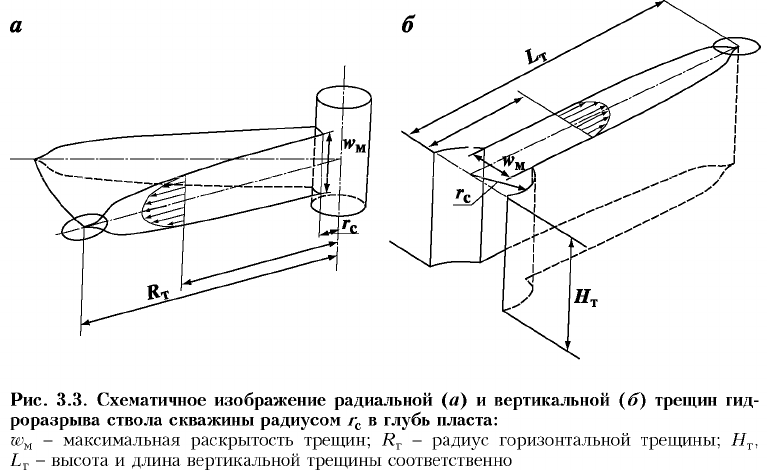
\includegraphics[height=0.4\textheight]{pictures/crack_g_v.png}
	\caption{ [1].
	}
	\label{fig:introduction1}
\end{figure}

\newpage
\section{Упругость}
\subsection{Уравнения равновесия}
В статьях \cite{Gupta2014,Gupta2015,Gupta2017,Duarte2019,Duarte2020_validation} используются уравнения равновесия
\begin{equation}
\int_{\Omega} \sigma:\varepsilon\,d\Omega=
\int_{\partial\Omega} \bar{t}\cdot v\,d\Gamma+
\int_{\Gamma_c^+} \bar{t}_c^+ \cdot \left(v^+-v^-\right)\,d\Gamma,
\label{F:F_XFEM_Governing}
\end{equation}
где $v$ -- пробная функция, $\bar{t}$ -- давление на границе тела $\Omega$, $v^+-v^-$ -- скачок перемещения через границу трещины, $\bar{t}_c^+=-\bar{t}_c^-$ -- давление на поверхность трещины.
\subsection{Базисные функциии}
В XFEM стандартный базис Лагранжа расширяется разрывными функциями:
\begin{equation}
\Delta \mathbf{u}^h\left(\mathbf{x}\right)=
\sum_{n\in N_{nodes}}\sum_{m\in M_{n}}\psi_{nm} \mathbf{a}_{nm},
%\sum_{n=1}^{N}\mathbf{q}_{nm}\varphi_{n}\left(\mathbf{x}\right)
%+\sum_{n=1}^{N}a_{(3n+k-3)}\varphi_{n}\left(\mathbf{x}\right)\left(H\left(\mathbf{x}\right)-H\left(\mathbf{x}_n\right)\right),
\label{F:F_XFEM_appr}
\end{equation}
\begin{equation}
\psi_{nm}=\varphi_n\left(\mathbf{x}\right)\psi_m\left(\mathbf{x}\right)
\label{F:F_XFEM_appr2}
\end{equation}
где $\varphi_{n}$ -- лагранжевы функции формы, $\psi_m\left(\mathbf{x}\right) = 1$ для базисных функций Лагранжа, $\psi_m\left(\mathbf{x}\right)=\psi_m^{enr}\left(\mathbf{x}\right)-\psi_m^{enr}\left(\mathbf{x}_n\right)$ для функций обогащения. $N_{nodes}$ -- множество узлов сетки, $M_{n}$ -- множество степеней свободы узла $n$ (по каждой из координат).

Для задания сильного разрыва вводится функция знака
\begin{equation}
\psi^{enr}=sgn\left(\mathbf{x}\right)=
\begin{cases}
-1 \: \mathrm{if} \: g\left(\mathbf{x}\right)<0\\
+1 \: \mathrm{if} \: g\left(\mathbf{x}\right)>0,\\
\end{cases}
\label{F:F_Hev}
\end{equation}
или Хевисайда
\begin{equation}
\psi^{enr}=H\left(\mathbf{x}\right)=
\begin{cases}
-1 \: \mathrm{if} \: g\left(\mathbf{x}\right)<0\\
0 \: \mathrm{if} \: g\left(\mathbf{x}\right)>0,\\
\end{cases}
\label{F:F_Hev2}
\end{equation}
что приводит к тому же результату. Случай нескольких трещин в одном КЭ рассмотрен в \cite{Moes2013,Moes2016,Moes2017,Paul2018}

Чтобы около фронта трещины в базисе содержалось точное решение линейно-упругой теории разрушения (LEFM), добавляются функции
\begin{equation}
\psi_m^{enr}\left(\mathbf{x}\right)\in\left\lbrace
\sqrt{r}\,\mathrm{sin}\frac{\theta}{2},
\sqrt{r}\,\mathrm{cos}\frac{\theta}{2},
\sqrt{r}\,\mathrm{sin}\frac{\theta}{2}\,\mathrm{sin}\theta,
\sqrt{r}\,\mathrm{cos}\frac{\theta}{2}\,\mathrm{sin}\theta\right\rbrace,
\label{F:F_Williams1}
\end{equation}
где $g\left(\mathbf{x}\right)$ -- функция расстояния от точки $\mathbf{x}$ до поверхности трещины (положительная с одной стороны трещины и отрицательная с другой стороны трещины); $r\left(\mathbf{x}\right)=\left| g\left(\mathbf{x}\right)\right|$; $\theta\left(\mathbf{x}\right)$ -- угол, под которым видна плоскость трещины из точки $\mathbf{x}$.

Функции \eqref{F:F_Williams1} получаются из асимптотического решения Вильямса \cite{Williams1961} и применялись в \cite{Belytschko1999} для XFEM. Эквивалентные альтернативы обогащений обсуждаются в \cite{Gupta2013,Gupta2015_sgfem}.

Функции обогащения для ортотропного материала: \cite{Asadpoure2007,Hattori2012}.

В смешанном подходе для упругопластического анализа трещин \cite{Feulvarch2020} вводится дополнительное поле давления и аппроксимирующие его функции около фронта трещины \cite{Westergaard1939}
\begin{equation}
\psi_m^{enr}\left(\mathbf{x}\right)\in\left\lbrace
\frac{1}{\sqrt{r}}\,\mathrm{cos}\frac{\theta}{2},
\frac{1}{\sqrt{r}}\,\mathrm{sin}\frac{\theta}{2},
\right\rbrace,
\label{F:F_Westergaard}
\end{equation}

\subsection{Интегрирование}
Разрывную функцию можно проинтегрировать по КЭ, разделив его на подобласти, на которых функция непрерывна, тогда можно будет применить квадратурные формулы Гаусса на каждой подобласти \cite{Fries2010,GuptaDiss2016,Weber2016}. Шестигранник можно разрезать на 5 тетраэдров (не единственным способом). Чтобы сгустить точки Гаусса к фронту трещины, тетраэдр можно интегрировать как шестигранник, используя отображение \cite{Minnebo2012}, или разбивать поверхность пересечения трещины с тетраэдром на тетраэдры \cite{GuptaDiss2016}. Разбиение шестигранника на призмы для случая вертикальной трещины с классификацией случаев рассмотрено в \cite{Nagashima2020}.

Другой подход, пригодный для интегрирования функций Хевисайда, основан на усреднении объёма и квадратурных формулах Гаусса \cite{Belytschko1988,Nikolakopoulos2020}.

\section{Рост трещины (LEFM)}
\subsection{Направление роста трещины}
Направление роста трещины можно задать при помощи угла в координатах фронта трещины: углом изгиба $\theta_0$ и углом закручивания $\varphi_0$ при помощи критерия максимума тангенциального напряжения Schollmann \cite{Schollmann2002}:
\begin{equation}
\left.\frac{\partial\sigma_1}{\partial\theta}=0\right|_{\theta=\theta_0},\,\left.\frac{\partial^2\sigma_1}{\partial\theta^2}<0\right|_{\theta=\theta_0},
\label{F:F_Schollmann1}
\end{equation}
\begin{equation}
\varphi_0=\frac{1}{2}\mathrm{arctan}\left( \frac{2\tau_{\theta z}\left(\theta_0 \right)}{\sigma_\theta\left(\theta_0 \right)-\sigma_z\left(\theta_0 \right)} \right),
\label{F:F_Schollmann2}
\end{equation}
где $\sigma_1$ -- максимальное главное напряжение; $\sigma_\theta$, $\tau_{\theta z}$ и $\sigma_\theta$ -- компоненты тензора напряжений в цилиндрической системе координат, заданной относительно фронта трещины.

Процедура вычисления эффективного направления $\theta^*$ с учётом углов $\theta_0$ и $\varphi_0$ дана в \cite{PereiraDiss2010}.
\subsection{Величина продвижения фронта при росте трещины}
В случае хрупкого разрушения, величину продвижения фронта (для некоторого узла) можно задать критерием Irwin \cite{Irwin1997} в регуляризованном виде, предложенном \cite{Lazarus2003}, который использовался в \cite{Gupta2017,Duarte2019,Duarte2020_validation,Duarte2020}:
\begin{equation}
\Delta a =
\begin{cases}
0, & \mathrm{}\;0\leqslant \frac{K_{I,eq}}{K_{Ic}} < 1-\alpha-\beta \\
\frac{\Delta a_{max}}{\beta}\left(  \frac{K_{I,eq}}{K_{Ic}} - \left( 1-\alpha-\beta \right) \right) , & \mathrm{}\;1-\alpha-\beta \leqslant \frac{K_{I,eq}}{K_{Ic}} < 1-\alpha \\
\Delta a_{max}, & \mathrm{}\;1-\alpha \leqslant \frac{K_{I,eq}}{K_{Ic}} \leqslant 1+\alpha \\
\end{cases}
\label{F:F_propogation1}
\end{equation}
где
\begin{equation}
\begin{gathered}
K_{I,eq} = \frac{1}{2}\mathrm{cos}\left( \frac{\theta_0}{2} \right)
\left(K_I\,\mathrm{cos}^2 \left(\frac{\theta_0}{2}\right)-\frac{3}{2}K_{II}\,\mathrm{sin} \left(\theta_0\right) \right. \\ 
\left. +\sqrt{\left(K_I\,\mathrm{cos}^2 \left(\frac{\theta_0}{2}\right)-\frac{3}{2}K_{II}\,\mathrm{sin} \left(\theta_0\right)\right)^2+4K_{III}^2}
\right),
\end{gathered}
\label{F:F_propogation2}
\end{equation}
$K_{I},\,K_{II},\,K_{III}$ -- коэффициенты интенсивностей напряжений (КИН, открывающая (I), поперечно-сдвиговая (II) и продольно-сдвиговая (III) моды деформаций), $K_{I,eq}$ -- эквивалентная мода I, $K_{Ic}$ -- трещиностойкость. $\alpha,\,\beta,\,\Delta a_{max}$ -- параметры материала.

В \cite{Gupta2014} применялись критерии
\begin{equation}
\Delta a =
\begin{cases}
0, & \mathrm{}\; K_{I,eq}\leqslant K_{Ic} \\
\Delta a_{max}\left(\frac{K_{I,eq}-K_{Ic}}{K_{I,eq}^{max}-K_{Ic}}\right)^m, & \mathrm{}\; K_{I,eq}>K_{Ic}\\
\end{cases}
\label{F:F_propogation3}
\end{equation}
и
\begin{equation}
\Delta a = \Delta a_{max}\left(\frac{K_{I,eq}}{K_{I,eq}^{max}}\right)^m
\label{F:F_propogation4}
\end{equation}
где $\Delta a_{max}$ и $m$ -- параметры материала.
\subsection{Вычисление SIF}
Сравнение методов вычисления КИН \cite{Gupta2017_SIF} показывает, что предпочтительным является Displacement Correlation Method (DCM), который основан на связи перемещений и КИН:
\begin{equation}
\begin{gathered}
K_{I,r}=\sqrt{\frac{2\pi}{r}}\left(\frac{\mu}{\kappa+1}\right)\Delta v\left(r\right), \\
K_{II,r}=\sqrt{\frac{2\pi}{r}}\left(\frac{\mu}{\kappa+1}\right)\Delta u\left(r\right), \\
K_{III,r}=\sqrt{\frac{2\pi}{r}}\left(\frac{\mu}{4}\right)\Delta w\left(r\right), \\
\end{gathered}
\label{F:DCM1}
\end{equation}
где $\kappa=3-4\nu$. $\Delta u,\,\Delta v,\,\Delta w$ -- компоненты скачка вектора перемещений ($\theta=\pm\pi$) в системе координат, связанной с фронтом трещины.
\begin{figure}[h!]
	\centering
	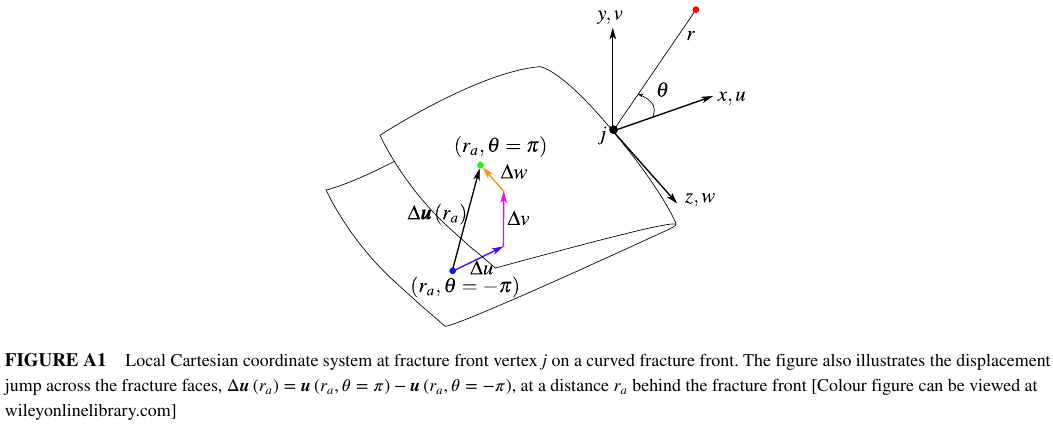
\includegraphics[height=0.2\textheight]{pictures/SIF.png}
	\caption{из \cite{Gupta2017}}
	\label{fig:SIF}
\end{figure}

Путём экстраполяции \cite{Dirgantara2002} можно получить КИН в вершине трещины:
\begin{equation}
\begin{gathered}
K_{I}=\frac{r_b}{r_b-r_a}\left(K_{I,r_a}-\frac{r_a}{r_b}K_{I,r_b}\right), \\
K_{II}=\frac{r_b}{r_b-r_a}\left(K_{II,r_a}-\frac{r_a}{r_b}K_{II,r_b}\right), \\
K_{III}=\frac{r_b}{r_b-r_a}\left(K_{III,r_a}-\frac{r_a}{r_b}K_{III,r_b}\right), \\
\end{gathered}
\label{F:DCM2}
\end{equation}
Этот метод наиболее просто реализовать. Требуется дробление сетки вблизи фронта трещины для обеспечения хорошей точности.
\section{Рост трещины (CZM)}
Модель сил сцепления (cohesive zone model) применялась в статьях \cite{Liu2016, Liu2017, Paul2018}, а также с использованием ABAQUS в статьях \cite{Zielonka2014, Haddad2016}.

Направление роста трещины задаётся формулами \eqref{F:F_Schollmann1}, \eqref{F:F_Schollmann2}.

Рост трещины в модели сил сцепления определяется силами сцепления $t_c$, действующими на поверхности трещины
\begin{equation}
t_c =
\begin{cases}
T_{ts}\frac{w}{g_0}, & \mathrm{}\; w\leqslant g_0 \\
T_{ts}\frac{g_1-w}{g_1-g_0} , & \mathrm{}\; g_0<w\leqslant g_1\\
0, & \mathrm{}\; w>g_1 \\
\end{cases}
\label{F:CZM}
\end{equation}
\begin{figure}[h!]
	\centering
	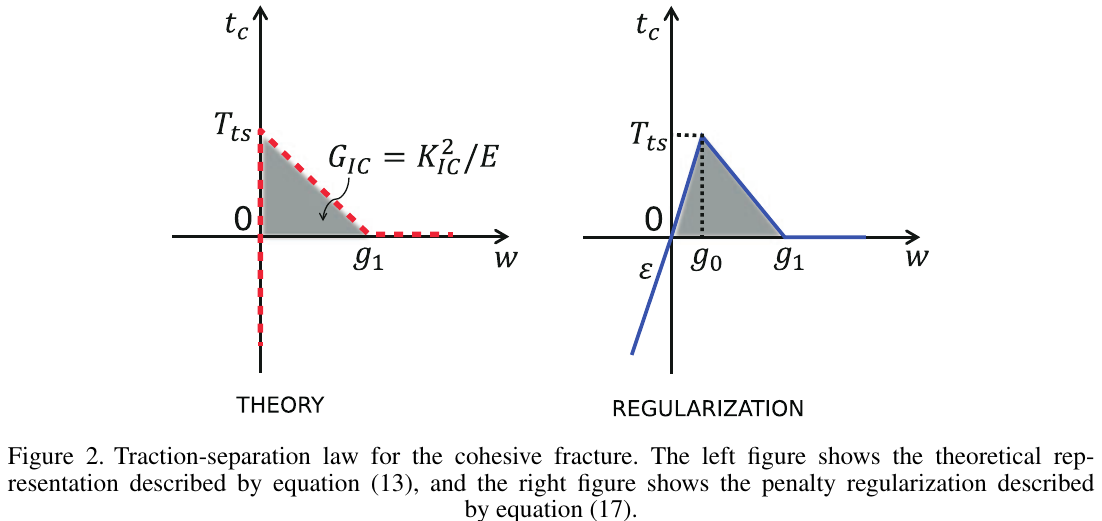
\includegraphics[height=0.3\textheight]{pictures/CZM_ts.png}
	\caption{из \cite{Liu2016}}
	\label{fig:CZM_ts}
\end{figure}
Связь параметра $g_2$ с вязкостью разрушения $K_{IC}$ определяется формулой \cite{Irwin1997}
\begin{equation}
K_{IC}=\sqrt{G_{IC}\frac{E}{1-\nu^2}}
\label{F:CZM1}
\end{equation}
где $G_{IC}$ -- энергии хрупкого разрушения:
\begin{equation}
G_{IC}=\frac{1}{2}T_{ts}g_1
\label{F:CZM2}
\end{equation}
Величина упругого участка $g_0$ считается малой:
\begin{equation}
g_0=\frac{T_{ts}}{\epsilon},\;\epsilon\gg E
\label{F:CZM3}
\end{equation}
Контакт между сторонами трещины автоматически учитывается дополнительным участком кривой при $w<0$.

В статьях \cite{Roth2020_1, Roth2020_2} в форме сил сцепления записана continuous damage model.

\section{Контакт, разветвление трещин, учёт природных трещин}
Для учёта контакта применимы стандартные методы типа штрафа \cite{GuptaDiss2016}.
Задание разветвлённых трещин (“junction” функции), взаимодействие между трещинами \cite{Moes2013,Moes2016,Moes2017,Paul2018}.
\section{Гидромеханика}
В статьях \cite{Gupta2015,Gupta2017,Duarte2019,Duarte2020} жидкость внутри трещины считается ньютоновской и несжимаемой, без учета инерционных и гравитационных эффектов, тогда закон сохранения массы приводит к уравнению
\begin{equation}
\int_{\Gamma_c}\left(\frac{\partial w}{\partial t}+q_L-q_I\right)v\,d\Gamma_c
-\int_{\Gamma_c}\mathbf{q}\cdot\nabla_{\overline{\mathbf{x}}}v\,d\Gamma_c
+\int_{\partial\Gamma_c^N}v\overline{q}\,ds=0
\label{F:F_flow1}
\end{equation}
где $w=\left(\mathbf{u}^+-\mathbf{u}^-\right)\cdot \mathbf{n}^-$ -- ширина трещины, $q_L$ -- утечка через границы трещины, $q_I$ -- скорость закачки жидкости, $v$ -- пробная функция, $\overline{q}$ -- поток по нормали к границе трещины $\partial\Gamma_c^N$, $\mathbf{q}$ -- поток внутри трещины, заданный кубическим законом Пуазейля
\begin{equation}
\mathbf{q} = -\frac{w^3}{12\mu}\nabla_{\overline{\mathbf{x}}}p,
\label{F:F_flow2}
\end{equation}
где $\mu$ -- вязкость жидкости,
\begin{equation}
\nabla_{\overline{\mathbf{x}}}=
 \frac{\partial}{\partial\overline{x}_1}\,\overline{\mathbf{e}}_1
+\frac{\partial}{\partial\overline{x}_2}\,\overline{\mathbf{e}}_2
\label{F:F_flow3}
\end{equation}
Каждая система координат с базовыми векторами $\left\lbrace \overline{\mathbf{e}}_1,\;\overline{\mathbf{e}}_2\right\rbrace $ и вектором положения $\left( \overline{x}_1,\;\overline{x}_2\right) $ связана с конечным элементом сетки, используемой для решения уравнения \eqref{F:F_flow1}.

\section{*Связанная гидро-механическая задача}
Gupta2017
?Дискретизация по времени
Пороупругость, leak-off Carter model (жидкость уходит в породу)
fluid lag (задержка жидкости из-за пористого включения в трещине)

Cohesive zone method (CZM), traction-separation constitutive law \cite{Moes2016}
viscosity- (M ) ... toughness- dominated (K) regime, GFEM enr.



\section{Сравнительный обзор статей}
\begin{landscape}
\begin{table}[h!]
	\caption{Обзор литературы}
	%\ctable [doinside=\small]
	%\begin{tabular}{|p{5.3cm}|c|p{7cm}|}
	%	\hline
	%	Параметр      & Обозначение & Значение  \\
	%	\hline
	%\begin{tabular}{|p{5.3cm}|c|p{7cm}|}
	%\small
	\footnotesize
	\begin{tabular}{|l|c|c|c|c|c|c|c|c|c|}
		\hline
		Источник & Год & Упругость & Обогащение & Рост трещины & Жидкость & Связанность & Разветвление & Контакт & Ком. CAE? \\
		\hline
		GD\cite{Gupta2014}&2014&упругость \eqref{F:F_XFEM_Governing}&Хевисайда, в вершине&Irwin \eqref{F:F_propogation3}, \eqref{F:F_propogation4} &$p=const$&---&---&---&---\\
		\hline
		GD\cite{Gupta2015}&2015&---//---&---//---&статика&\eqref{F:F_flow1}&м. Ньютона-Рафсона&---&---&---\\
		\hline
		GD\cite{Gupta2017}&2017&---//---&---//---&Irwin \eqref{F:F_propogation1}&\eqref{F:F_flow1}&м. Ньютона-Рафсона&---&---&---\\
		\hline
		GD\cite{Duarte2019}&2019&---//---&---//---&Irwin \eqref{F:F_propogation1}&\eqref{F:F_flow1}&м. Ньютона-Рафсона&---&---&---\\
		\hline
		GD\cite{Duarte2020_validation}&2020&---//---&---//---&Irwin \eqref{F:F_propogation3}&---&---&---&---&---\\
		\hline
		GD\cite{Duarte2020}&2020&---//---&---//---&Irwin \eqref{F:F_propogation1}&\eqref{F:F_flow1}&м. Ньютона-Рафсона&---&---&---\\
		\hline
		
		%CZM
		Liu\cite{Liu2016}&2016&упругость \eqref{F:F_XFEM_Governing}&Хевисайда&CZM \eqref{F:CZM}&\eqref{F:F_flow1}&м. Ньютона-Рафсона&---&включён в CZM&---\\
		\hline
		Liu\cite{Liu2017}&2017&упругость \eqref{F:F_XFEM_Governing}&Хевисайда&CZM \eqref{F:CZM}&\eqref{F:F_flow1}&м. Ньютона-Рафсона&---&включён в CZM&---\\
		\hline		
		\cite{Paul2018}&2018&пороупругость&Хевисайда, junction&CZM без рег.&\eqref{F:F_flow1}&расш. м. Лагранжа&разветвление&&---\\
		\hline
		
		
		\cite{Luo2018}&2018&&&&&&&&---\\
		\hline
%		Diss\cite{WeberDiss2016}&2016&&&&&&&&---\\
%		\hline

		Roth\cite{Roth2020_1}&2020&пороупругость&Хевисайда&CDM ч/з $t_c$&...&м. Ньютона-Рафсона&---&м. штрафа&---\\
		\hline
		Roth\cite{Roth2020_2}&2020&пороупругость&Хевисайда&CDM ч/з $t_c$&...&м. Ньютона-Рафсона&---&м. штрафа&---\\
		\hline

		%CZM ABAQUS 
		\cite{Zielonka2014}&2014&пороупругость&Хевисайда, ф. узлы&CZM \eqref{F:CZM}&\eqref{F:F_flow1}&&---&---&ABAQUS\\
		\hline
		\cite{Haddad2016}&2016&пороупругость&Хевисайда, ф. узлы&CZM \eqref{F:CZM}&&&пересечение&---&ABAQUS\\
		\hline
		

		
		
		\hline
	\end{tabular}
	\label{tab:lit_owerview}
\end{table}

\end{landscape}


%\newpage




%Неплоское распространение трещин в трехмерном пространстве, смоделированное с помощью XFEM, было представлено в %[Gupta2014]




%%% Local Variables:
%%% mode: latex
%%% TeX-master: "rpz"
%%% End:

\chapter{XFEM}
\label{cha:analysis}
\section{Постановка задачи}
В области $\Omega$ заданы уравнения равновесия \cite{Pisarenko1981}
\begin{equation}
%\sum\limits_{j=1}^{3} \frac{\partial\sigma_{ij}}{\partial x_j} = 0, i=\overline{1,3}.
%\frac{\partial\sigma_{ij}}{\partial x_j} = 0, i=\overline{1,3}.
%\bigtriangledown_j\sigma_{ij} = 0.%, i=\overline{1,3}.
\frac{\partial\sigma_{ij}}{\partial x_j} = 0.%, i=\overline{1,3}.
\label{F:F1}
\end{equation}
На границе $S=S_{1}\cup S_{2}$ заданы кинематические и силовые
краевые условия
\begin{equation}
\left.\mathbf{u}\right|_{S_{1}}=\mathbf{u}_{0}\left(t\right),
\label{F:F2}
\end{equation}
\begin{equation}
%\left.\sum\limits_{j=1}^{3}\sigma_{ij}n_j\right|_{S_{2}}=P_{i}\left(t\right),\:i=\overline{1,3},
\left.\sigma_{ij}n_j\right|_{S_{2}}=P_{i}\left(t,\,\mathbf{u}\right),% i=\overline{1,3},
\label{F:F3}
\end{equation}
где $\mathbf{u}$ --- вектор перемещения, $\mathbf{n}$ --- внешняя единичная нормаль к поверхности $S_{2}$, $\mathbf{P}$ --- вектор поверхностных сил.

Компоненты тензора малых деформаций Коши $\varepsilon$ связаны с перемещениями линейными геометрическими соотношениями
\begin{equation}
\varepsilon_{ij}=\frac{1}{2} \left(\frac{\partial u_{i}}{\partial x_{j}} + \frac{\partial u_{j}}{\partial x_{i}} \right).
\label{F:F4}
\end{equation}

Для изотропного тела тензор напряжений Коши $\sigma$ выражается через упругую составляющую $\varepsilon^{e}$ малой деформации Коши обобщенным законом Гука
\begin{equation}
%\sigma_{ij}=\sum\limits_{l=1}^{3} \sum\limits_{k=1}^{3} C_{ijkl}\varepsilon_{kl}^{e},
%\sigma_{ij}=C_{ijkl}\varepsilon_{kl}^{e},
\sigma=C:\varepsilon^{e},
\label{F:F_Hook}
\end{equation}
\begin{equation}
C_{ijkl}=\lambda\delta_{ij}\delta_{kl}+\mu\left(\delta_{ik}\delta_{jl}+\delta_{il}\delta_{jk}\right),
\label{F:F5}
\end{equation}
где $C$ --- тензор модулей упругости материала, $\lambda$, $\mu$ --- модули упругости Ламэ, $\delta$ --- символ Кронекера. Символом \textquotedblleft $:$\textquotedblright\ обозначено двойное скалярное произведение, т.е. $\left(C:\varepsilon\right)_{ij}\equiv C_{ijkl}\varepsilon_{kl}$.




\section{Дискретизация}
Домножим уравнения \eqref{F:F1} на пробную функцию $\upsilon$, применим формулу Грина интегрирования по частям и учтём силовые краевые условия \eqref{F:F3}, в результате система вариационных уравнений в форме Галеркина примет вид \cite{SoloveychikRoyakPersova2007}
\begin{equation}
\int\limits_{\Omega}\sigma_{ij}\frac{\partial\upsilon}{\partial x_j}  d\Omega=\int\limits_{S_{2}}P_{i} \upsilon dS.
\label{F:F_var2}
\end{equation}

Согласно шаговому методу для случая малых деформаций \cite{Zienkiewicz1975,Frolov1995}, для некоторого шага по времени $t\longrightarrow t+\Delta t$ запишем уравнение \eqref{F:F_var2} в приращениях

\begin{equation}
\int\limits_{\Omega}\Delta\sigma_{ij}\frac{\partial\upsilon}{\partial x_j} d\Omega=\int\limits_{S_{2}}\Delta P_{i} \upsilon dS + R_{i},
\label{F:F_var3}
\end{equation}
\begin{equation}
R_{i} \equiv \int\limits_{S_{2}}{}^{(t)}P_{i} \upsilon dS - \int\limits_{\Omega}{}^{(t)}\sigma_{ij}\frac{\partial\upsilon}{\partial x_j} d\Omega.
\label{F:F_var3_add}
\end{equation}

Подставим закон Гука \eqref{F:F_Hook} в приращениях
\begin{equation}
\Delta\sigma=C:\Delta\varepsilon
\label{F:F_alg_ce1}
\end{equation}
и \eqref{F:F4} (для приращений) в левую часть \eqref{F:F_var3} и, воспользовавшись симметрией \mbox{${C}_{ijkl}={C}_{ijlk}$}, получим 
\begin{equation}
\int\limits_{\Omega}{C}_{ijkl} \frac{\partial \Delta u_{k}}{\partial x_{l}} \frac{\partial\upsilon}{\partial x_j}d\Omega=\int\limits_{S_{2}}\Delta P_{i}\upsilon dS
+R_{i}.
\label{F:F_alg_var1}
\end{equation}

Перейдём к конечномерному пространству, натянутому на базисные функции $\left\lbrace\psi_{n}|\,n=\overline{1,N}\right\rbrace$, разложим компоненты приращения
\begin{equation}
\Delta u_k^h=\sum_{n=1}^{N}q_{(3n+k-3)}\psi_n,
\label{F:F_alg_var2}
\end{equation}
подставим вместо $\upsilon$ поочерёдно функции $\psi_{n}$ при $n=\overline{1,N}$, получим СЛАУ (здесь все суммирования записаны явно)
\begin{equation}
\begin{gathered}
\sum_{n=1}^{N}\sum_{j=1}^{3}\sum_{k=1}^{3}\sum_{l=1}^{3}
\int\limits_{\Omega}{C}_{ijkl}q_{(3n+k-3)} \frac{\partial \psi_{n}}{\partial x_{l}} \frac{\partial\psi_{m}}{\partial x_j}d\Omega= \\
\int\limits_{S_{2}}\Delta P_{i}\psi_{m} dS
+\left.R_{i}\right|_{\upsilon=\psi_{m}},
\end{gathered}
\label{F:F_alg_slau1}
\end{equation}
которую можно записать в виде
\begin{equation}
\mathbf{Gq}=\mathbf{b},
\label{F:F_slau2}
\end{equation}
где элементы матрицы жёсткости $\mathbf{G}$ и вектора $\mathbf{b}$ представимы в виде
\begin{equation}
G_{(3m+i-3)(3n+k-3)}=\int\limits_{\Omega}{C}_{ijkl}\frac{\partial\psi_{m}}{\partial x_j}\frac{\partial \psi_{n}}{\partial x_{l}}d\Omega,
\label{F:F_slau3}
\end{equation}
\begin{equation}
b_{(3m+i-3)}=
\int\limits_{S_{2}}\Delta P_{i}\psi_{m} dS
+R_{(3m+i-3)}^{\mathrm{node}},
\label{F:F_slau4}
\end{equation}

\begin{equation}
R_{(3m+i-3)}^{\mathrm{node}} \equiv \int\limits_{S_{2}}{}^{(t)}P_{i} \psi_{m} dS - \int\limits_{\Omega}{}^{(t)}\sigma_{ij}\frac{\partial\psi_{m}}{\partial x_j} d\Omega.
\label{F:F_slau4_add}
\end{equation}

\section{Интегрирование}
Рассмотрим некоторый шестигранный КЭ $\Omega_K$. Отображение шаблонного куба $\Omega^E=[-1,1]^3$ в шестигранник $\Omega_K$ с заданными координатами вершин $\hat{\mathbf{x}}_i$ задаётся соотношениями
\begin{equation}
\mathbf{x}\left(\bm{\xi}\right)=\sum_{i=1}^{8}\hat{\varphi}_i\left(\bm{\xi}\right)\hat{\mathbf{x}}_i,
\label{F:F_mapping}
\end{equation}
где $\hat{\varphi}_i\left(\bm{\xi}\right)$ -- трилинейные базисные функции на шаблонном кубе  $\Omega^E$:
\begin{equation}
\hat{\varphi}_i\left(\bm{\xi}\right)=
Q_{\beta_1(i)}\left(\xi_1\right)
Q_{\beta_2(i)}\left(\xi_2\right)
Q_{\beta_3(i)}\left(\xi_3\right),
\: i=1\ldots 8
\label{F:F_mapping_linear1}
\end{equation}
\begin{equation}
\begin{gathered}
Q_1\left(\alpha\right)=\left(1-\alpha\right)/2, \: 
Q_2\left(\alpha\right)=\left(1+\alpha\right)/2, \\
\beta_1(i)=\left(\left(i-1\right) \mathrm{mod} \: 2\right)+1, \\
\beta_2(i)=\left(\left[\left(i-1\right)/2\right] \mathrm{mod} \: 2\right)+1, \\
\beta_3(i)=\left[\left(i-1\right)/4\right]+1.
\end{gathered}
\label{F:F_mapping_linear2}
\end{equation}
Локальные базисные функции можно задать в координатах шаблонного куба:
\begin{equation}
\hat{\psi}_{n}=\hat{\psi}_{n}\left(\bm{\xi}\right)
\label{F:F_mapping_linear3}
\end{equation}

Разделим шестигранник $\Omega_K$ на шестигранные подобласти, которые не пересекаются трещиной. Пусть некоторый шестигранник $\omega_k$ (подобласть) задан координатами шаблонного куба $\hat{\bm{\xi}}_i$. Тогда координаты вершин шестигранника $\omega_k$ определяются отображением \eqref{F:F_mapping}
\begin{equation}
\hat{\hat{\mathbf{x}}}_j=\sum_{i=1}^{8}\hat{\varphi}_i\left(\hat{\bm{\xi}}_j\right)\hat{\mathbf{x}}_i,\: j=1\ldots 8
\label{F:F_sub_vertexes}
\end{equation}
Аналогично \eqref{F:F_mapping}, зададим отображение из шаблонного куба в шестигранник $\omega_k$:
\begin{equation}
\mathbf{x}\left(\bm{\eta}\right)=\sum_{i=1}^{8}\hat{\varphi}_i\left(\bm{\eta}\right)\hat{\hat{\mathbf{x}}}_i,
\label{F:F_sub_mapping}
\end{equation}
Базисные функции в подобласти $\omega_k$ зададим интерполянтом в координатах шаблонного куба
\begin{equation}
\hat{\hat{\psi}}_n\left(\bm{\eta}\right)=\sum_{i=1}^{8}\hat{\varphi}_i\left(\bm{\eta}\right)
\hat{\psi}_n\left(\hat{\bm{\xi}}_i\right).
\label{F:F_sub_busfuncvalues}
\end{equation}
Для нахождения производных в выражении
\begin{equation}
\int\limits_{\omega_k}\frac{\partial\hat{\hat{\psi}}_{m}}{\partial x_j}\frac{\partial\hat{\hat{\psi}}_{n}}{\partial x_{l}}d\Omega
\label{F:F_sub_int1}
\end{equation}
воспользуемся правилом интегрирования сложной функции
\begin{equation}
\left(
\begin{array}{c}
\frac{\partial\hat{\hat{\psi}}_{m}}{\partial\eta_1} \\
\frac{\partial\hat{\hat{\psi}}_{m}}{\partial\eta_2} \\
\frac{\partial\hat{\hat{\psi}}_{m}}{\partial\eta_3} 
\end{array}
\right)
=
\mathbf{J}
\left(
\begin{array}{c}
\frac{\partial\hat{\hat{\psi}}_{m}}{\partial x_1} \\
\frac{\partial\hat{\hat{\psi}}_{m}}{\partial x_2} \\
\frac{\partial\hat{\hat{\psi}}_{m}}{\partial x_3} 
\end{array}
\right)
\label{F:F_sub_dif1}
\end{equation}

\begin{equation}
\mathbf{J}=
\left(
\begin{array}{ccc}
\frac{\partial x_1}{\partial \eta_1} & \frac{\partial x_2}{\partial \eta_1} & \frac{\partial x_3}{\partial \eta_1}\\
\frac{\partial x_1}{\partial \eta_2} & \frac{\partial x_2}{\partial \eta_2} & \frac{\partial x_3}{\partial \eta_2}\\
\frac{\partial x_1}{\partial \eta_3} & \frac{\partial x_2}{\partial \eta_3} & \frac{\partial x_3}{\partial \eta_3}
\end{array}
\right),
\label{F:F_sub_dif2}
\end{equation}
где $\mathbf{J}$ -- якобиан отображения \eqref{F:F_sub_mapping} шаблонного куба в шестигранник $\omega_k$.
Тогда 
\begin{equation}
\int\limits_{\omega_k}\frac{\partial\hat{\hat{\psi}}_{m}}{\partial x_j}\frac{\partial\hat{\hat{\psi}}_{n}}{\partial x_{l}}d\Omega
=\int\limits_{-1}^{1}\int\limits_{-1}^{1}\int\limits_{-1}^{1}
\frac{\partial\hat{\hat{\psi}}_{m}}{\partial x_j}
\frac{\partial\hat{\hat{\psi}}_{n}}{\partial x_{l}}\left| \mathbf{J} \right|d\eta_1d\eta_2d\eta_3
\label{F:F_sub_int2}
\end{equation}
Для интегрирования по поверхности трещины
\begin{equation}
\int\limits_{S_{k}^+}\Delta P_{i}^+\psi_{m} dS+
\int\limits_{S_{k}^-}\Delta P_{i}^-\psi_{m} dS
\label{F:F_sub_int3}
\end{equation}
имеем
\begin{equation}
\int\limits_{s_k^+}\hat{\hat{\psi}}_{m}ds
=\int\limits_{-1}^{1}\int\limits_{-1}^{1}
\hat{\hat{\psi}}_{m}\left| \mathbf{J} \right|d\eta_1d\eta_2
\label{F:F_sub_int4}
\end{equation}


\section{Пластинка с трещиной}
Параллелепипед с трещиной растягивается вдоль оси $x$ (рис. \ref{fig:grid}). Параметры задачи приведены в таблице \ref{tab:test1_parameters}. Пластинка закреплена в плоскостях $x = -4, y = -4, z = 0$ по осям $x, y, z$ соответственно, и имеет 3 слоя с различными модулями Юнга (границы слоёв $y=-1, y=1$). К стороне $x=4$ приложены поверхностные силы. Сравнение решений FEM и XFEM изображены на рисунках \ref{fig:res1}, \ref{fig:res2}. На графиках приведены решения, в которых обогащаются узлы 2-х слоёв шестигранников вокруг вершины трещины (XFEM) и решения, в которых обогащается только один слой (XFEM1). Решения различаются не значительно.
\begin{table}[h!]
	\caption{Параметры задачи}
	%\ctable [doinside=\small]
	
	%\begin{tabular}{|p{5.3cm}|c|p{7cm}|}
	%	\hline
	%	Параметр      & Обозначение & Значение  \\
	%	\hline
	\begin{tabular}{|p{5.3cm}|c|p{7cm}|}
		
		\hline
		Параметр & Обозначение & Значение \\
		\hline
		Модуль Юнга & $E_1, E_2, E_3$& $10^{6}, 2\cdot 10^{6}, 3\cdot 10^{6}$ Па \\
		\hline
		Коэффициент Пуассона & $\nu$ & $0.4$ \\
		\hline
		Размеры &  & $8\times 8\times 2$ м\\
		\hline
		Разбиение &  & $32\times 32\times 2$ \\
		\hline
		Давление на границе справа &  &$-5\cdot 10^3$ Па \\
		\hline
		Координаты трещины&  &$-0.85<y<0.85, -1<y<1$\\
		\hline
	\end{tabular}
	\label{tab:test1_parameters}
\end{table}
\begin{figure}[h!]
	\centering
	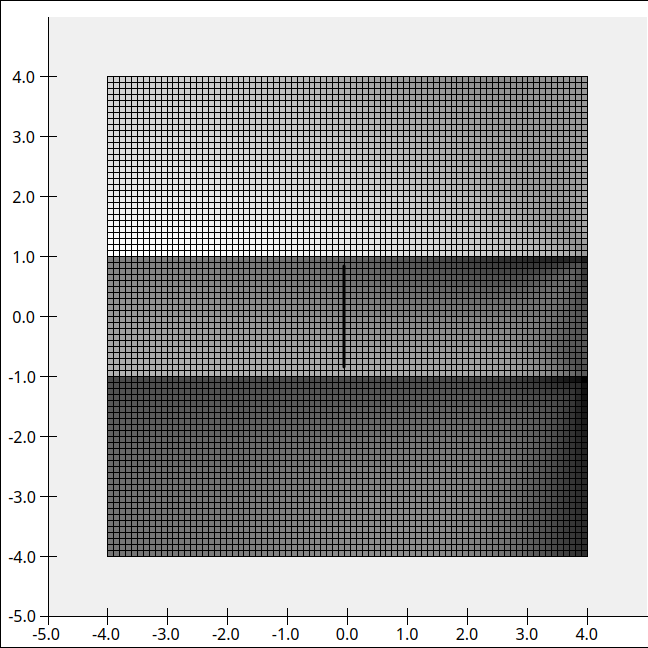
\includegraphics[height=0.3\textheight]{pictures/grid.png}
	\caption{ Сетка
	}
	\label{fig:grid}
\end{figure}
\begin{figure}[h!]
	%\centering
	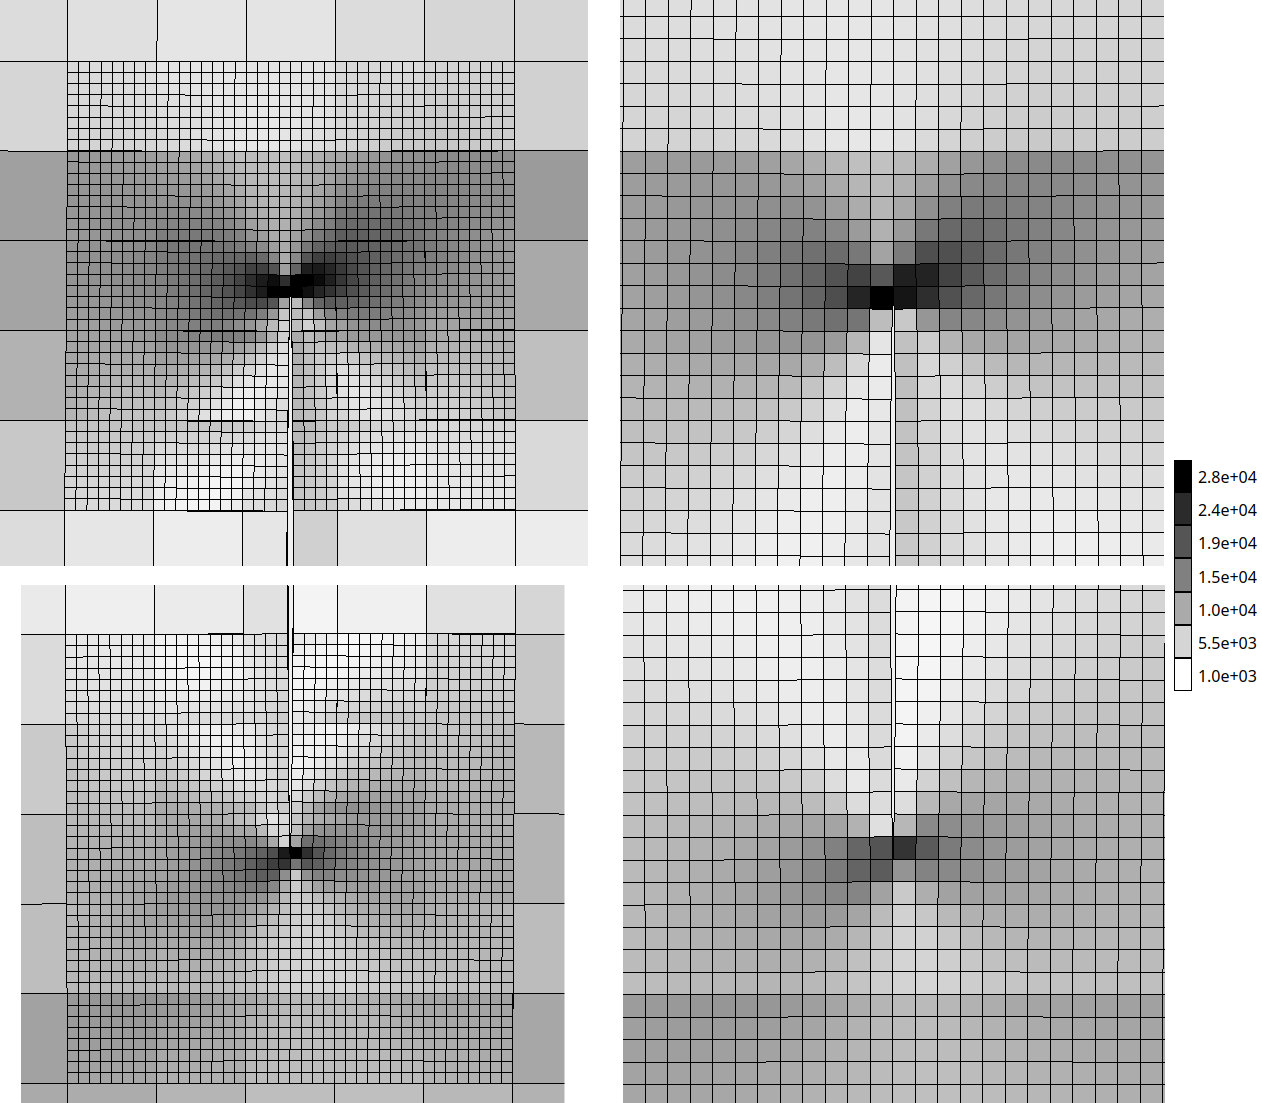
\includegraphics[height=0.4\textheight]{pictures/0.85_top_bot}
	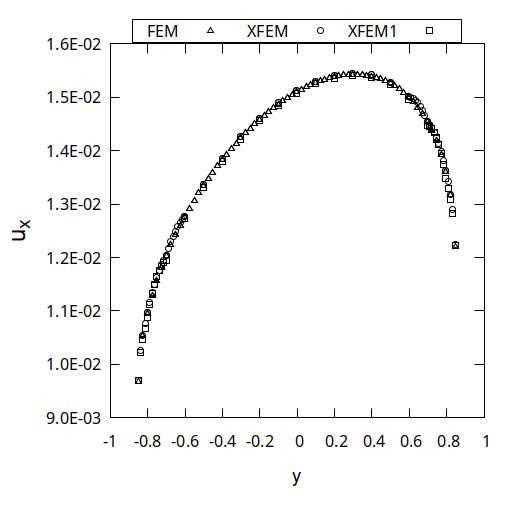
\includegraphics[height=0.4\textheight]{pictures/0.85_ux}
	\caption{ Трещина $-0.85<y<0.85$. Сверху показаны эквивалентные напряжения (слева XFEM, справа FEM). На графике показано сравнение перемещений по оси $x$ в правой части трещины. Напряжения в XFEM достигали значения $3.8\cdot 10^{4}$.
	}
	\label{fig:res1}
\end{figure}
\begin{figure}[h!]
	%\centering
	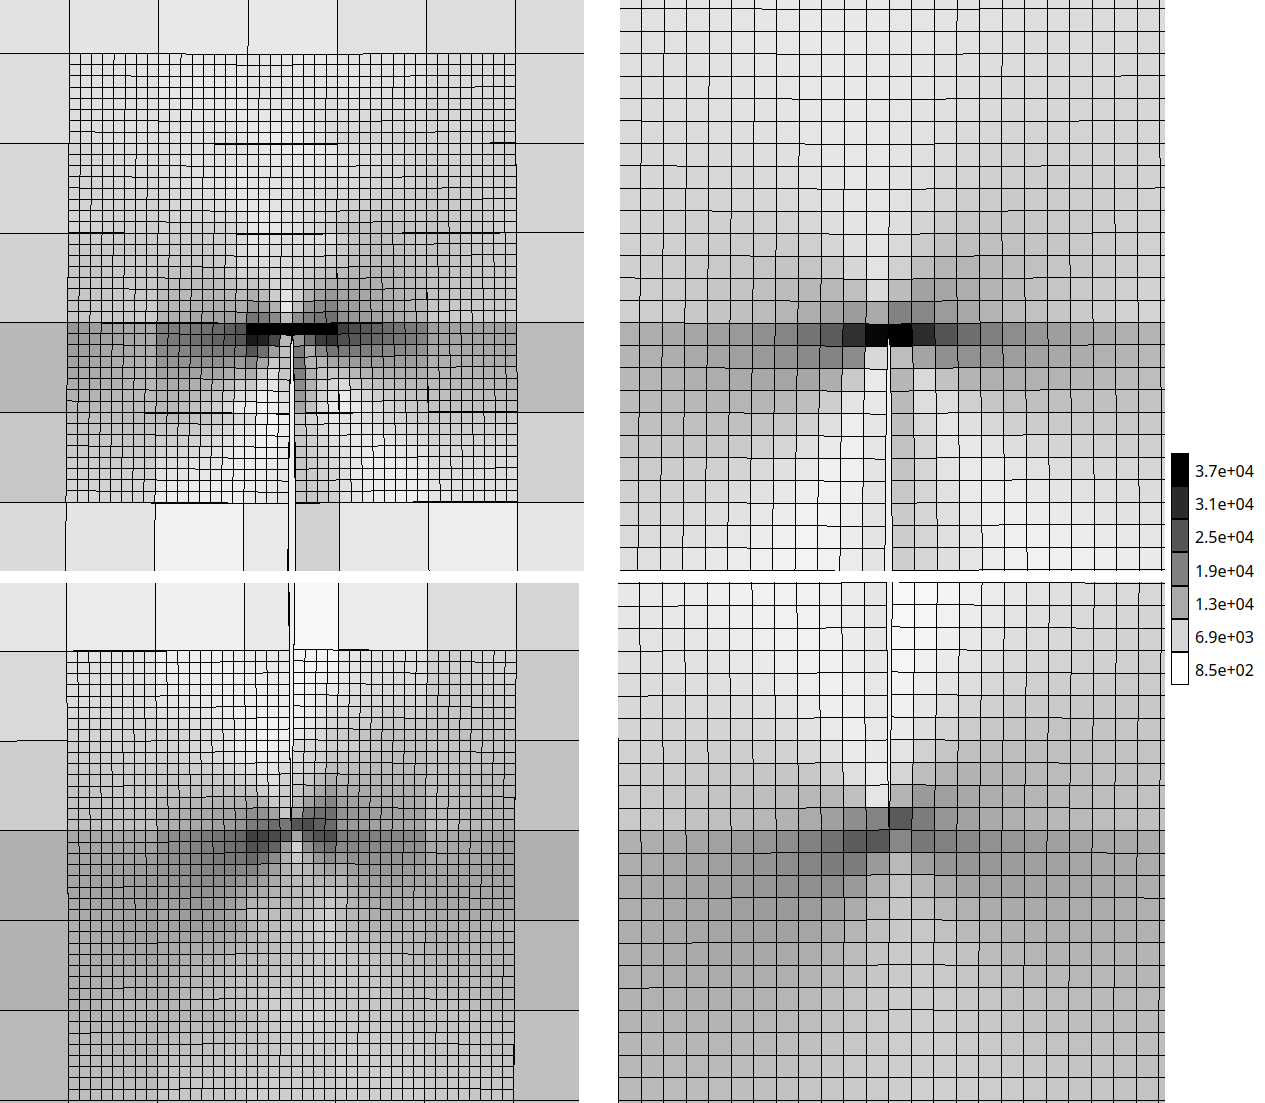
\includegraphics[height=0.4\textheight]{pictures/1.0_top_bot}
	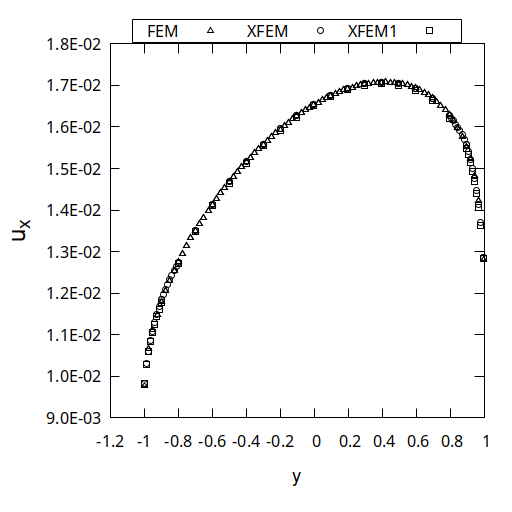
\includegraphics[height=0.4\textheight]{pictures/1.0_ux}
	\caption{ Трещина $-1<y<1$. Сверху показаны эквивалентные напряжения (слева XFEM, справа FEM). На графике показано сравнение перемещений по оси $x$ в правой части трещины. Напряжения в XFEM достигали значения $4.3\cdot 10^{4}$.
	}
	\label{fig:res2}
\end{figure}
\begin{figure}[h!]
	%\centering
	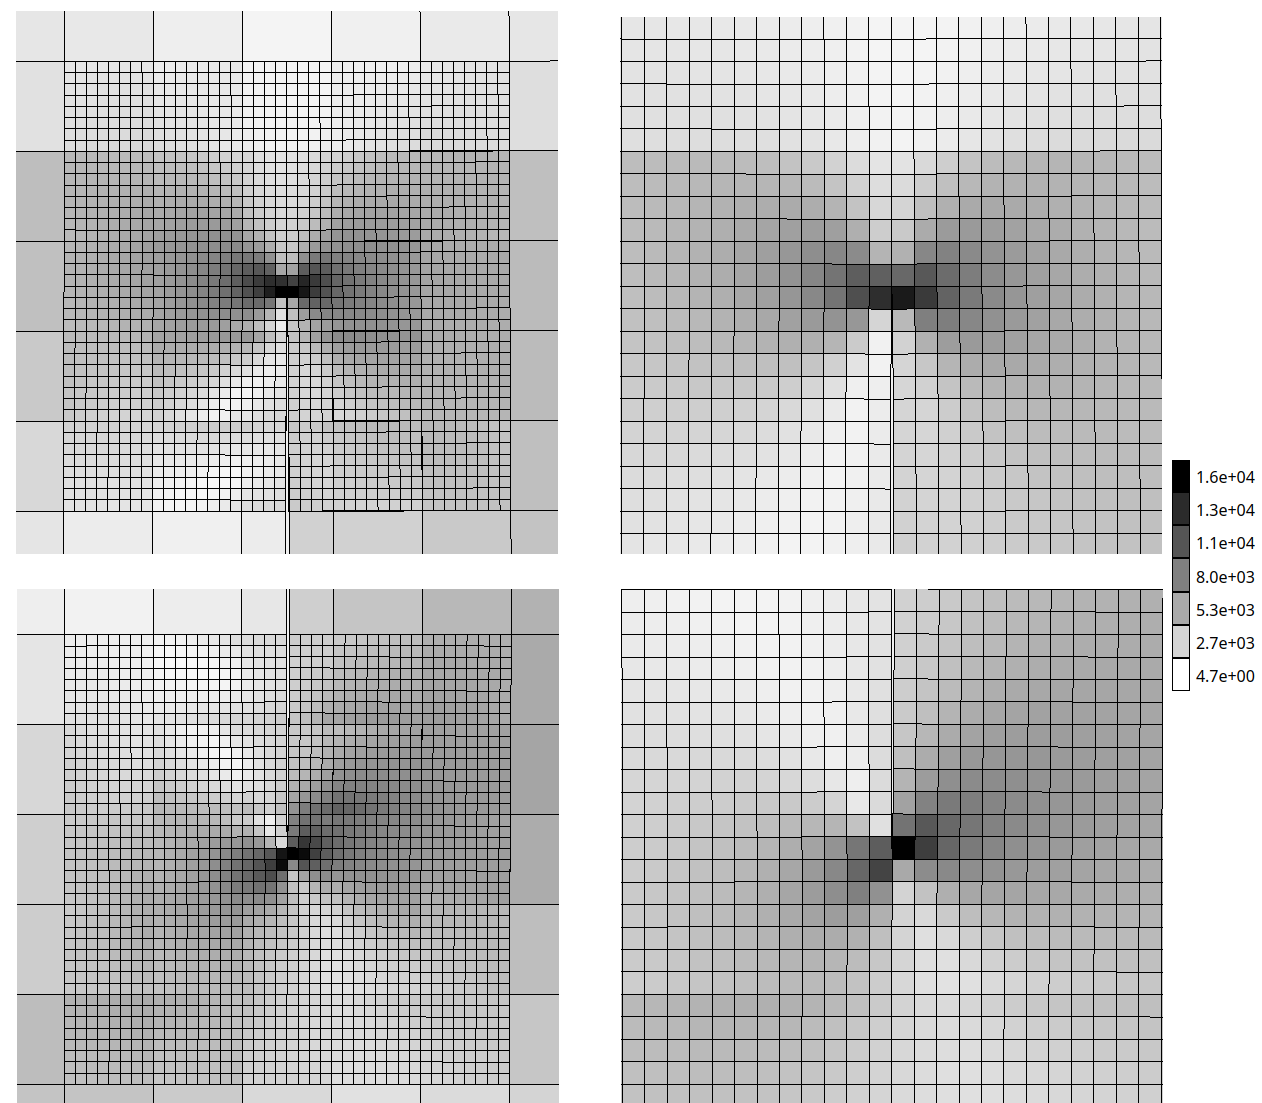
\includegraphics[height=0.4\textheight]{pictures/bc2_0.85_top_bot}
	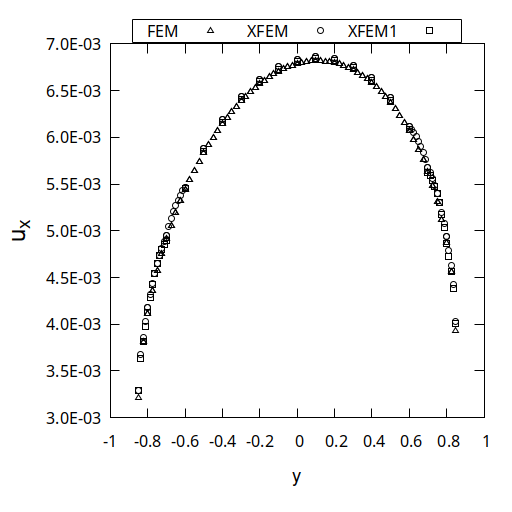
\includegraphics[height=0.4\textheight]{pictures/bc2_0.85_ux}
	\caption{ Трещина $-0.85<y<0.85$, давление приложено к правой части трещины. Сверху показаны эквивалентные напряжения (слева XFEM, справа FEM). На графике показано сравнение перемещений по оси $x$ в правой части трещины. Напряжения в XFEM достигали значения $2.0\cdot 10^{4}$.
	}
	\label{fig:res3}
\end{figure}

%%% Local Variables:
%%% mode: latex
%%% TeX-master: "rpz"
%%% End:


\begin{thebibliography}{3}
\bibitem{Magadova2012}
Магадова Л. А., Силин М. А., Глущенко В. Н. Нефтепромысловая химия. Технологические аспекты и материалы для гидроразрыва пласта //издательский центр РГУ нефти и газа им. ИМ Губина учебное пособие.–2012.–423 с. – 2012.


\bibitem{GuptaDiss2016}
Gupta P. A generalized finite element method for the simulation of non-planar three-dimensional hydraulic fracture propagation : дис. – University of Illinois at Urbana-Champaign, 2016.
\bibitem{WeberDiss2016}
Weber N. The XFEM for Hydraulic Fracture Mechanics Die XFEM für die hydraulische Bruchmechanik.
\bibitem{Lecampion2018}
Lecampion B., Bunger A., Zhang X. Numerical methods for hydraulic fracture propagation: a review of recent trends //Journal of natural gas science and engineering. – 2018. – Т. 49. – С. 66-83.
\bibitem{Kolawole2020}
Kolawole O., Ispas I. Interaction between hydraulic fractures and natural fractures: current status and prospective directions //Journal of Petroleum Exploration and Production Technology. – 2020. – Т. 10. – №. 4. – С. 1613-1634.

\bibitem{PereiraDiss2010}
Pereira J. P. Generalized finite element methods for three-dimensional crack growth simulations : дис. – University of Illinois at Urbana-Champaign, 2010.
\bibitem{Belytschko2009}
Belytschko T., Gracie R., Ventura G. A review of extended/generalized finite element methods for material modeling //Modelling and Simulation in Materials Science and Engineering. – 2009. – Т. 17. – №. 4. – С. 043001.
\bibitem{Fries2010}
Fries T. P., Belytschko T. The extended/generalized finite element method: an overview of the method and its applications //International journal for numerical methods in engineering. – 2010. – Т. 84. – №. 3. – С. 253-304.
\bibitem{Karihaloo2011}
Karihaloo B., Xiao Q. Z. Accurate simulation of mixed-mode cohesive crack propagation in quasi-brittle structures using exact asymptotic fields in XFEM: an overview //Journal of Mechanics of Materials and Structures. – 2011. – Т. 6. – №. 1. – С. 267-276.
\bibitem{Fries2014}
Fries T. P. Overview and comparison of different variants of the XFEM //PAMM. – 2014. – Т. 14. – №. 1. – С. 27-30.
\bibitem{flemisch2016}
Flemisch B., Fumagalli A., Scotti A. A review of the XFEM-based approximation of flow in fractured porous media //Advances in Discretization Methods. – 2016. – С. 47-76.
\bibitem{Ahmadkanth2019}
Kanth S. A. et al. Elasto Plastic Crack Growth by XFEM: A Review //Materials Today: Proceedings. – 2019. – Т. 18. – С. 3472-3481.

\bibitem{Gupta2014}
Gupta P., Duarte C. A. Simulation of non‐planar three‐dimensional hydraulic fracture propagation //International Journal for Numerical and Analytical Methods in Geomechanics. – 2014. – Т. 38. – №. 13. – С. 1397-1430.
\bibitem{Zielonka2014}
Zielonka M. G. et al. Development and validation of fully-coupled hydraulic fracturing simulation capabilities //Proceedings of the SIMULIA community conference, SCC2014. – 2014. – С. 19-21.
\bibitem{Gupta2015}
Gupta P., Duarte C. A. Coupled formulation and algorithms for the simulation of non-planar three-dimensional hydraulic fractures using the generalized finite element method //International Journal for Numerical and Analytical Methods in Geomechanics. – 2016. – Т. 40. – №. 10. – С. 1402-1437.
\bibitem{Liu2016}
Liu F. et al. A stabilized extended finite element framework for hydraulic fracturing simulations //International Journal for Numerical and Analytical Methods in Geomechanics. – 2017. – Т. 41. – №. 5. – С. 654-681.
\bibitem{Weber2016}
Weber N. The XFEM for Hydraulic Fracture Mechanics Die XFEM für die hydraulische Bruchmechanik.
\bibitem{Haddad2016}
Haddad M., Sepehrnoori K. XFEM-based CZM for the simulation of 3D multiple-cluster hydraulic fracturing in quasi-brittle shale formations //Rock Mechanics and Rock Engineering. – 2016. – Т. 49. – №. 12. – С. 4731-4748.
\bibitem{Gupta2017}
Gupta P., Duarte C. A. Coupled hydromechanical‐fracture simulations of nonplanar three‐dimensional hydraulic fracture propagation //International Journal for Numerical and Analytical Methods in Geomechanics. – 2018. – Т. 42. – №. 1. – С. 143-180.
\bibitem{Liu2017}
Liu F., Gordon P. A., Valiveti D. M. Modeling competing hydraulic fracture propagation with the extended finite element method //Acta Geotechnica. – 2018. – Т. 13. – №. 2. – С. 243-265.
\bibitem{Luo2018}
Luo Z. et al. Seepage-stress coupling mechanism for intersections between hydraulic fractures and natural fractures //Journal of Petroleum Science and Engineering. – 2018. – Т. 171. – С. 37-47.
\bibitem{Paul2018}
Paul B. et al. 3D coupled HM–XFEM modeling with cohesive zone model and applications to non planar hydraulic fracture propagation and multiple hydraulic fractures interference //Computer Methods in Applied Mechanics and Engineering. – 2018. – Т. 342. – С. 321-353.
\bibitem{Duarte2019}
Shauer N., Duarte C. A. Improved algorithms for generalized finite element simulations of three‐dimensional hydraulic fracture propagation //International Journal for Numerical and Analytical Methods in Geomechanics. – 2019. – Т. 43. – №. 18. – С. 2707-2742.
\bibitem{Duarte2020_validation}
Mukhtar F. M., Alves P. D., Duarte C. A. Validation of a 3-D adaptive stable generalized/eXtended finite element method for mixed-mode brittle fracture propagation //International Journal of Fracture. – 2020. – Т. 225. – №. 2. – С. 129-152.
\bibitem{Duarte2020}
Shauer N., Duarte C. A. A generalized finite element method for three-dimensional hydraulic fracture propagation: Comparison with experiments //Engineering Fracture Mechanics. – 2020. – Т. 235. – С. 107098.
\bibitem{Roth2020_1}
Roth S. N., Léger P., Soulaïmani A. Strongly coupled XFEM formulation for non-planar three-dimensional simulation of hydraulic fracturing with emphasis on concrete dams //Computer Methods in Applied Mechanics and Engineering. – 2020. – Т. 363. – С. 112899.
\bibitem{Roth2020_2}
Roth S. N., Léger P., Soulaïmani A. Fully-coupled hydro-mechanical cracking using XFEM in 3D for application to complex flow in discontinuities including drainage system //Computer Methods in Applied Mechanics and Engineering. – 2020. – Т. 370. – С. 113282.
\bibitem{Shi2021}
??Shi F., Liu J. A fully coupled hydromechanical XFEM model for the simulation of 3D non-planar fluid-driven fracture propagation //Computers and Geotechnics. – 2021. – Т. 132. – С. 103971.

\bibitem{Williams1961}
Williams M. L. The bending stress distribution at the base of a stationary crack. – 1961.
\bibitem{Moes2012}
Geniaut S., Massin P., Moës N. A stable 3D contact formulation using X-FEM //European Journal of Computational Mechanics/Revue Européenne de Mécanique Numérique. – 2007. – Т. 16. – №. 2. – С. 259-275.
\bibitem{Moes2013}
Siavelis M. et al. Large sliding contact along branched discontinuities with X-FEM //Computational mechanics. – 2013. – Т. 52. – №. 1. – С. 201-219.
\bibitem{Moes2016}
Ferté G., Massin P., Moës N. 3D crack propagation with cohesive elements in the extended finite element method //Computer Methods in Applied Mechanics and Engineering. – 2016. – Т. 300. – С. 347-374.
\bibitem{Moes2017}
Paul B. et al. An integration technique for 3D curved cracks and branched discontinuities within the extended Finite Element Method //Finite Elements in Analysis and Design. – 2017. – Т. 123. – С. 19-50.
\bibitem{Belytschko1999}
Belytschko T., Black T. Elastic crack growth in finite elements with minimal remeshing //International journal for numerical methods in engineering. – 1999. – Т. 45. – №. 5. – С. 601-620.
\bibitem{Gupta2013}
Gupta V. et al. A stable and optimally convergent generalized FEM (SGFEM) for linear elastic fracture mechanics //Computer methods in applied mechanics and engineering. – 2013. – Т. 266. – С. 23-39.
\bibitem{Gupta2015_sgfem}
Gupta V. et al. Stable GFEM (SGFEM): Improved conditioning and accuracy of GFEM/XFEM for three-dimensional fracture mechanics //Computer methods in applied mechanics and engineering. – 2015. – Т. 289. – С. 355-386.
\bibitem{Asadpoure2007}
Asadpoure A., Mohammadi S. Developing new enrichment functions for crack simulation in orthotropic media by the extended finite element method //International Journal for Numerical Methods in Engineering. – 2007. – Т. 69. – №. 10. – С. 2150-2172.
\bibitem{Hattori2012}
Hattori G. et al. New anisotropic crack-tip enrichment functions for the extended finite element method //Computational Mechanics. – 2012. – Т. 50. – №. 5. – С. 591-601.
\bibitem{Feulvarch2020}
Feulvarch E., Lacroix R., Deschanels H. A 3D locking-free XFEM formulation for the von Mises elasto-plastic analysis of cracks //Computer Methods in Applied Mechanics and Engineering. – 2020. – Т. 361. – С. 112805.
\bibitem{Westergaard1939}
??Westergaard H. M. Bearing pressures and cracks //Trans AIME, J. Appl. Mech. – 1939. – Т. 6. – С. 49-53.
\bibitem{Minnebo2012}
Minnebo H. Three‐dimensional integration strategies of singular functions introduced by the XFEM in the LEFM //International Journal for Numerical Methods in Engineering. – 2012. – Т. 92. – №. 13. – С. 1117-1138.
\bibitem{Nagashima2020}
NAGASHIMA T. Three-dimensional crack analyses under thermal stress field by XFEM using only the Heaviside step function //Mechanical Engineering Journal. – 2020. – Т. 7. – №. 4. – С. 20-00098-20-00098.
\bibitem{Belytschko1988}
Belytschko T., Fish J., Engelmann B. E. A finite element with embedded localization zones //Computer methods in applied mechanics and engineering. – 1988. – Т. 70. – №. 1. – С. 59-89.
\bibitem{Nikolakopoulos2020}
Nikolakopoulos K., Crete J. P., Longère P. Volume averaging based integration method in the context of XFEM-cohesive zone model coupling //Mechanics Research Communications. – 2020. – Т. 104. – С. 103485.


\bibitem{Schollmann2002}
Schollmann M. et al. A new criterion for the prediction of crack development in multiaxially loaded structures //International Journal of Fracture. – 2002. – Т. 117. – №. 2. – С. 129-141.
\bibitem{Irwin1997}
Irwin G. R. Analysis of stresses and strains near the end of a crack traversing a plate. – 1997.
\bibitem{Lazarus2003}
Lazarus V. Brittle fracture and fatigue propagation paths of 3D plane cracks under uniform remote tensile loading //International journal of Fracture. – 2003. – Т. 122. – №. 1. – С. 23-46.
\bibitem{Gupta2017_SIF}
Gupta P., Duarte C. A., Dhankhar A. Accuracy and robustness of stress intensity factor extraction methods for the generalized/eXtended Finite Element Method //Engineering Fracture Mechanics. – 2017. – Т. 179. – С. 120-153.
\bibitem{Dirgantara2002}
Dirgantara T., Aliabadi M. H. Stress intensity factors for cracks in thin plates //Engineering fracture mechanics. – 2002. – Т. 69. – №. 13. – С. 1465-1486.


\bibitem{Pisarenko1981}
Писаренко Г. С., Можаровский Н. С. Уравнения и краевые задачи теории пластичности и ползучести. --- Киев : Наукова думка, 1981. --- 496 с.
\bibitem{SoloveychikRoyakPersova2007}
Соловейчик Ю. Г., Рояк М. Э., Персова М. Г. Метод конечных элементов для решения скалярных и векторных задач. --- Новосибирск : Изд-­во НГТУ, 2007. --- 895 с.
\bibitem{Zienkiewicz1975}
Зенкевич О. Метод конечных элементов в технике. --- М. : Мир, 1975. --- 542 с.
\bibitem{Frolov1995}
Александров А. В., Алфутов Н. А., Астанин В. В. и др. Энциклопедия ”Машиностроение”. Том I-­3. ”Динамика и прочность машин. Теория механизмов и машин”. В 2-­х книгах. Кн. 2 / Под ред. Фролов К. В. (гл. ред.). --- М. : Машиностроение, 1995. --- 624 с.
\bibitem{Khoei2014}
Khoei A. R. Extended finite element method: theory and applications. – John Wiley \& Sons, 2014.
	
\end{thebibliography}

%%% Local Variables:
%%% mode: latex
%%% TeX-master: "rpz"
%%% End:




% \iffalse
% \include{20-analysis}
% \fi

 
% \include{30-design}
% \include{40-impl}
% \include{50-research}
% \include{60-economics}
% \include{70-bzd}

\backmatter %% Здесь заканчивается нумерованная часть документа и начинаются ссылки и
            
% \include{80-conclusion}%% заключение




\appendix   % Тут идут приложения

% \include{90-appendix1}

% \include{91-appendix2}


%\fi

\end{document}

%%% Local Variables:
%%% mode: latex
%%% TeX-master: t
%%% End:
